%!TEX root = ../../../adrien_gomar_phd.tex

The mesh considered to compute this
CROR configuration is a single-blade passage meshed
with an O4H topology show in Fig.~\ref{fig:dream_mesh}. This is a classical
topology for turbomachinery computations that is here applied to 
a CROR.
\begin{figure}[htb]
  \centering
  \subfigure[Topology]{
    \label{fig:dream_mesh}
    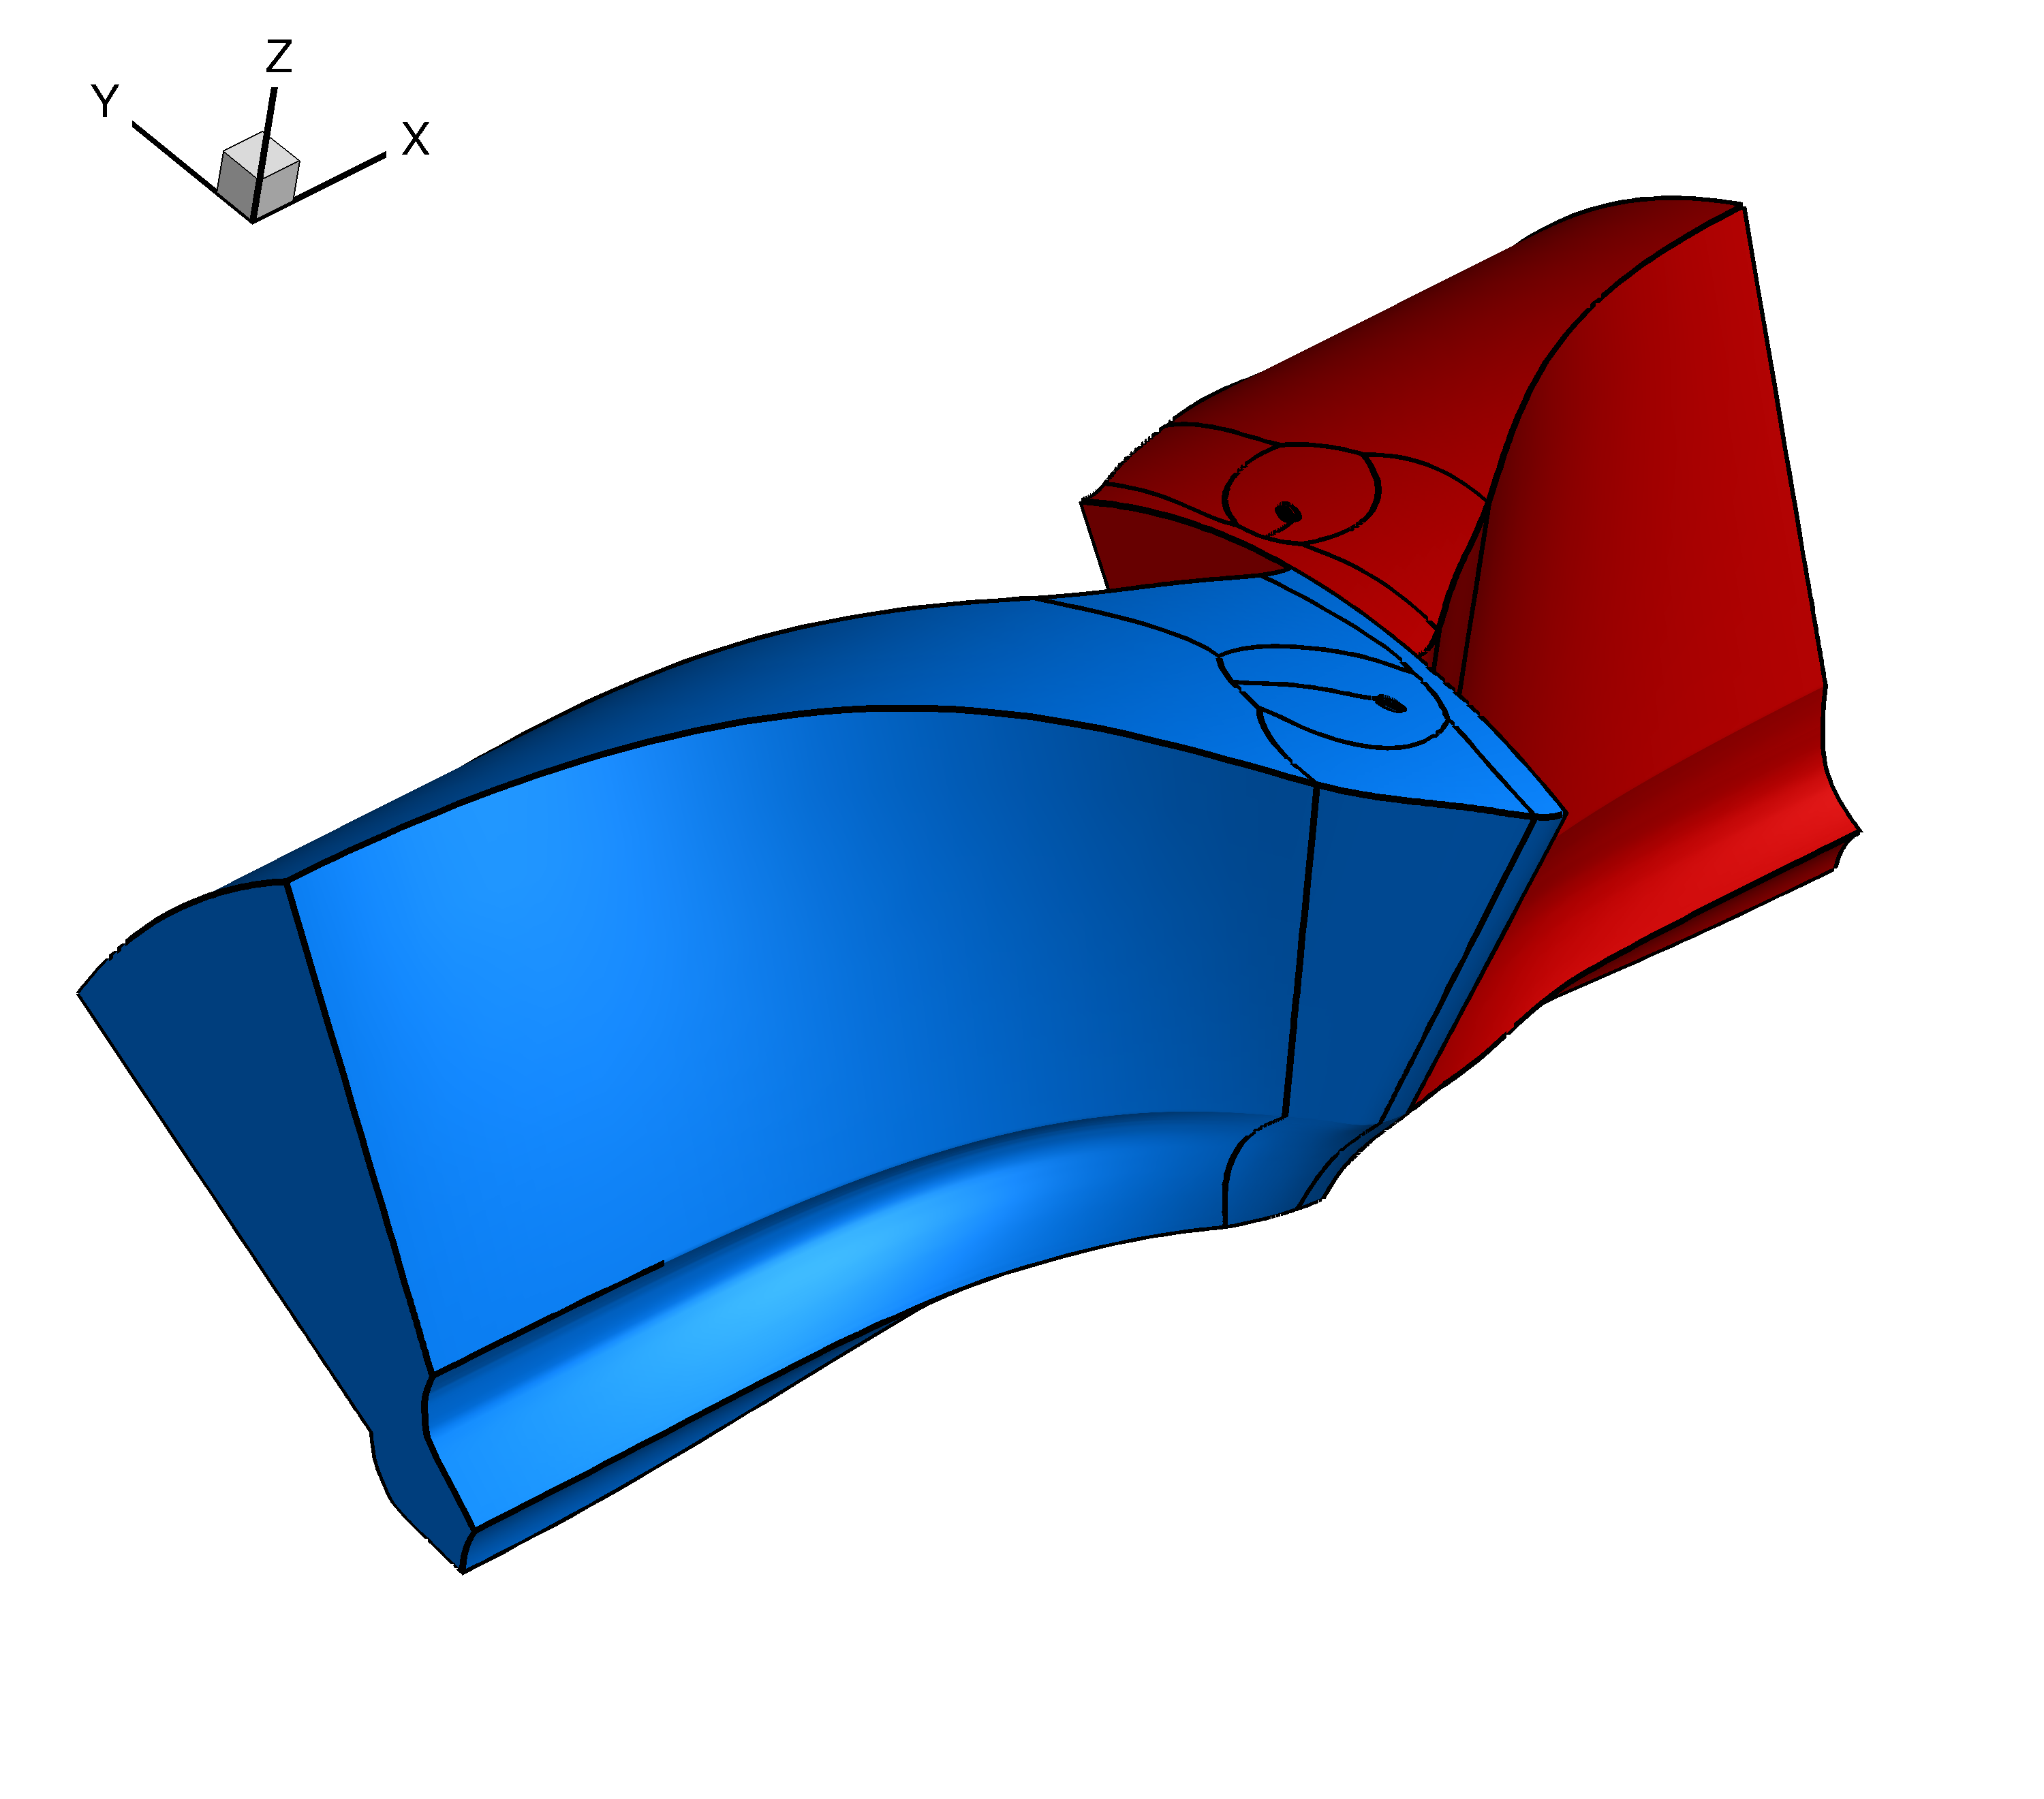
\includegraphics[height=.4\textwidth]{dream_mesh.png}}
  \subfigure[Detailed topology with number of grid points]{
    \label{fig:dream_ls_mesh}
    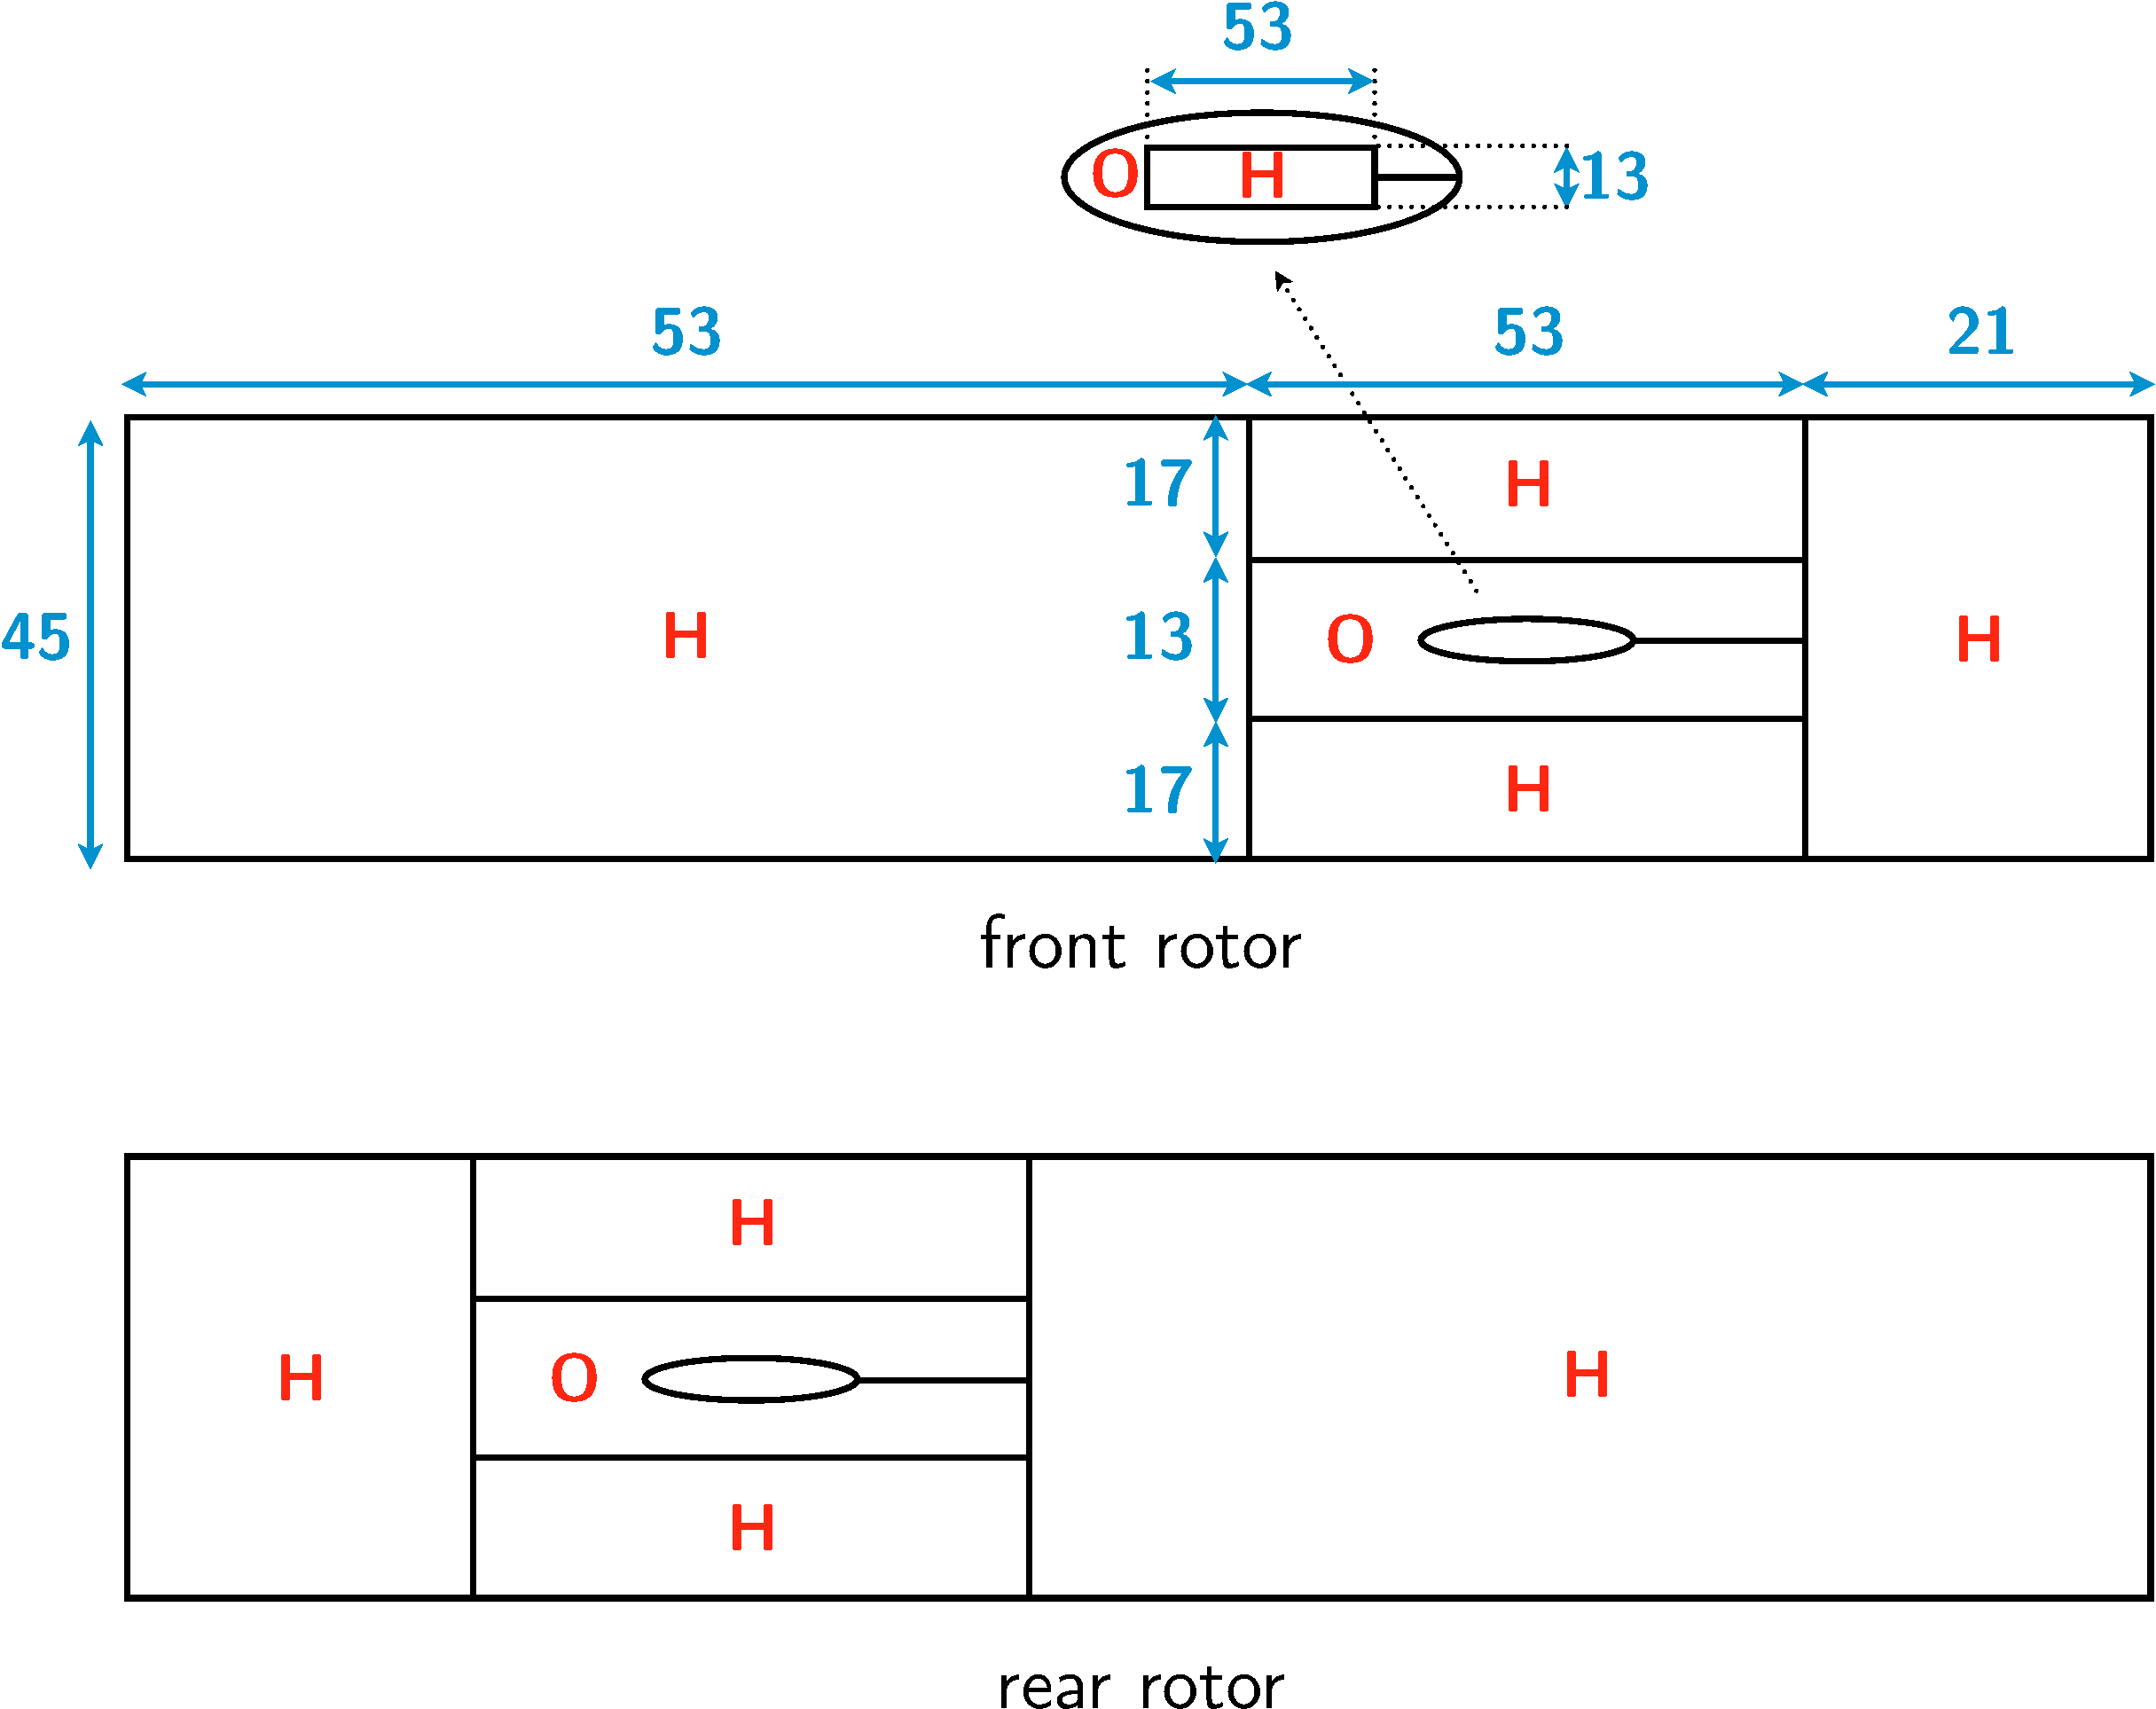
\includegraphics[height=.4\textwidth]{dream_ls_mesh.pdf}}
  \caption{Low-speed isolated configuration mesh topology.}
\end{figure}
The number of points is reported in 
Fig.~\ref{fig:dream_ls_mesh} for a blade-to-blade section. 
129~points discretize the blade, 45~the pitch and 181~the radial
extent. The same number of points is used for the front
and the rear rotors. These number of grid points are
classical inputs for steady RANS computations.

As a CROR is not shrouded, a sufficiently large
far-field domain is taken to ensure a minimum influence
of the far-field boundary conditions on the results.
The computational domain is shown in Fig.~\ref{fig:dream_farfield}.
The radial extent is $3D$ while the axial one is $3.5D$.
\citet{Peters2012} consider an axial extent of $7.5D$
with a radial extent of $4D$ while \citet{Zachariadis2011}
consider $2.5D$ and $3.6D$, respectively. We are thus in 
the mid-range of the values taken in the literature.
\begin{figure}[htb]
  \centering
  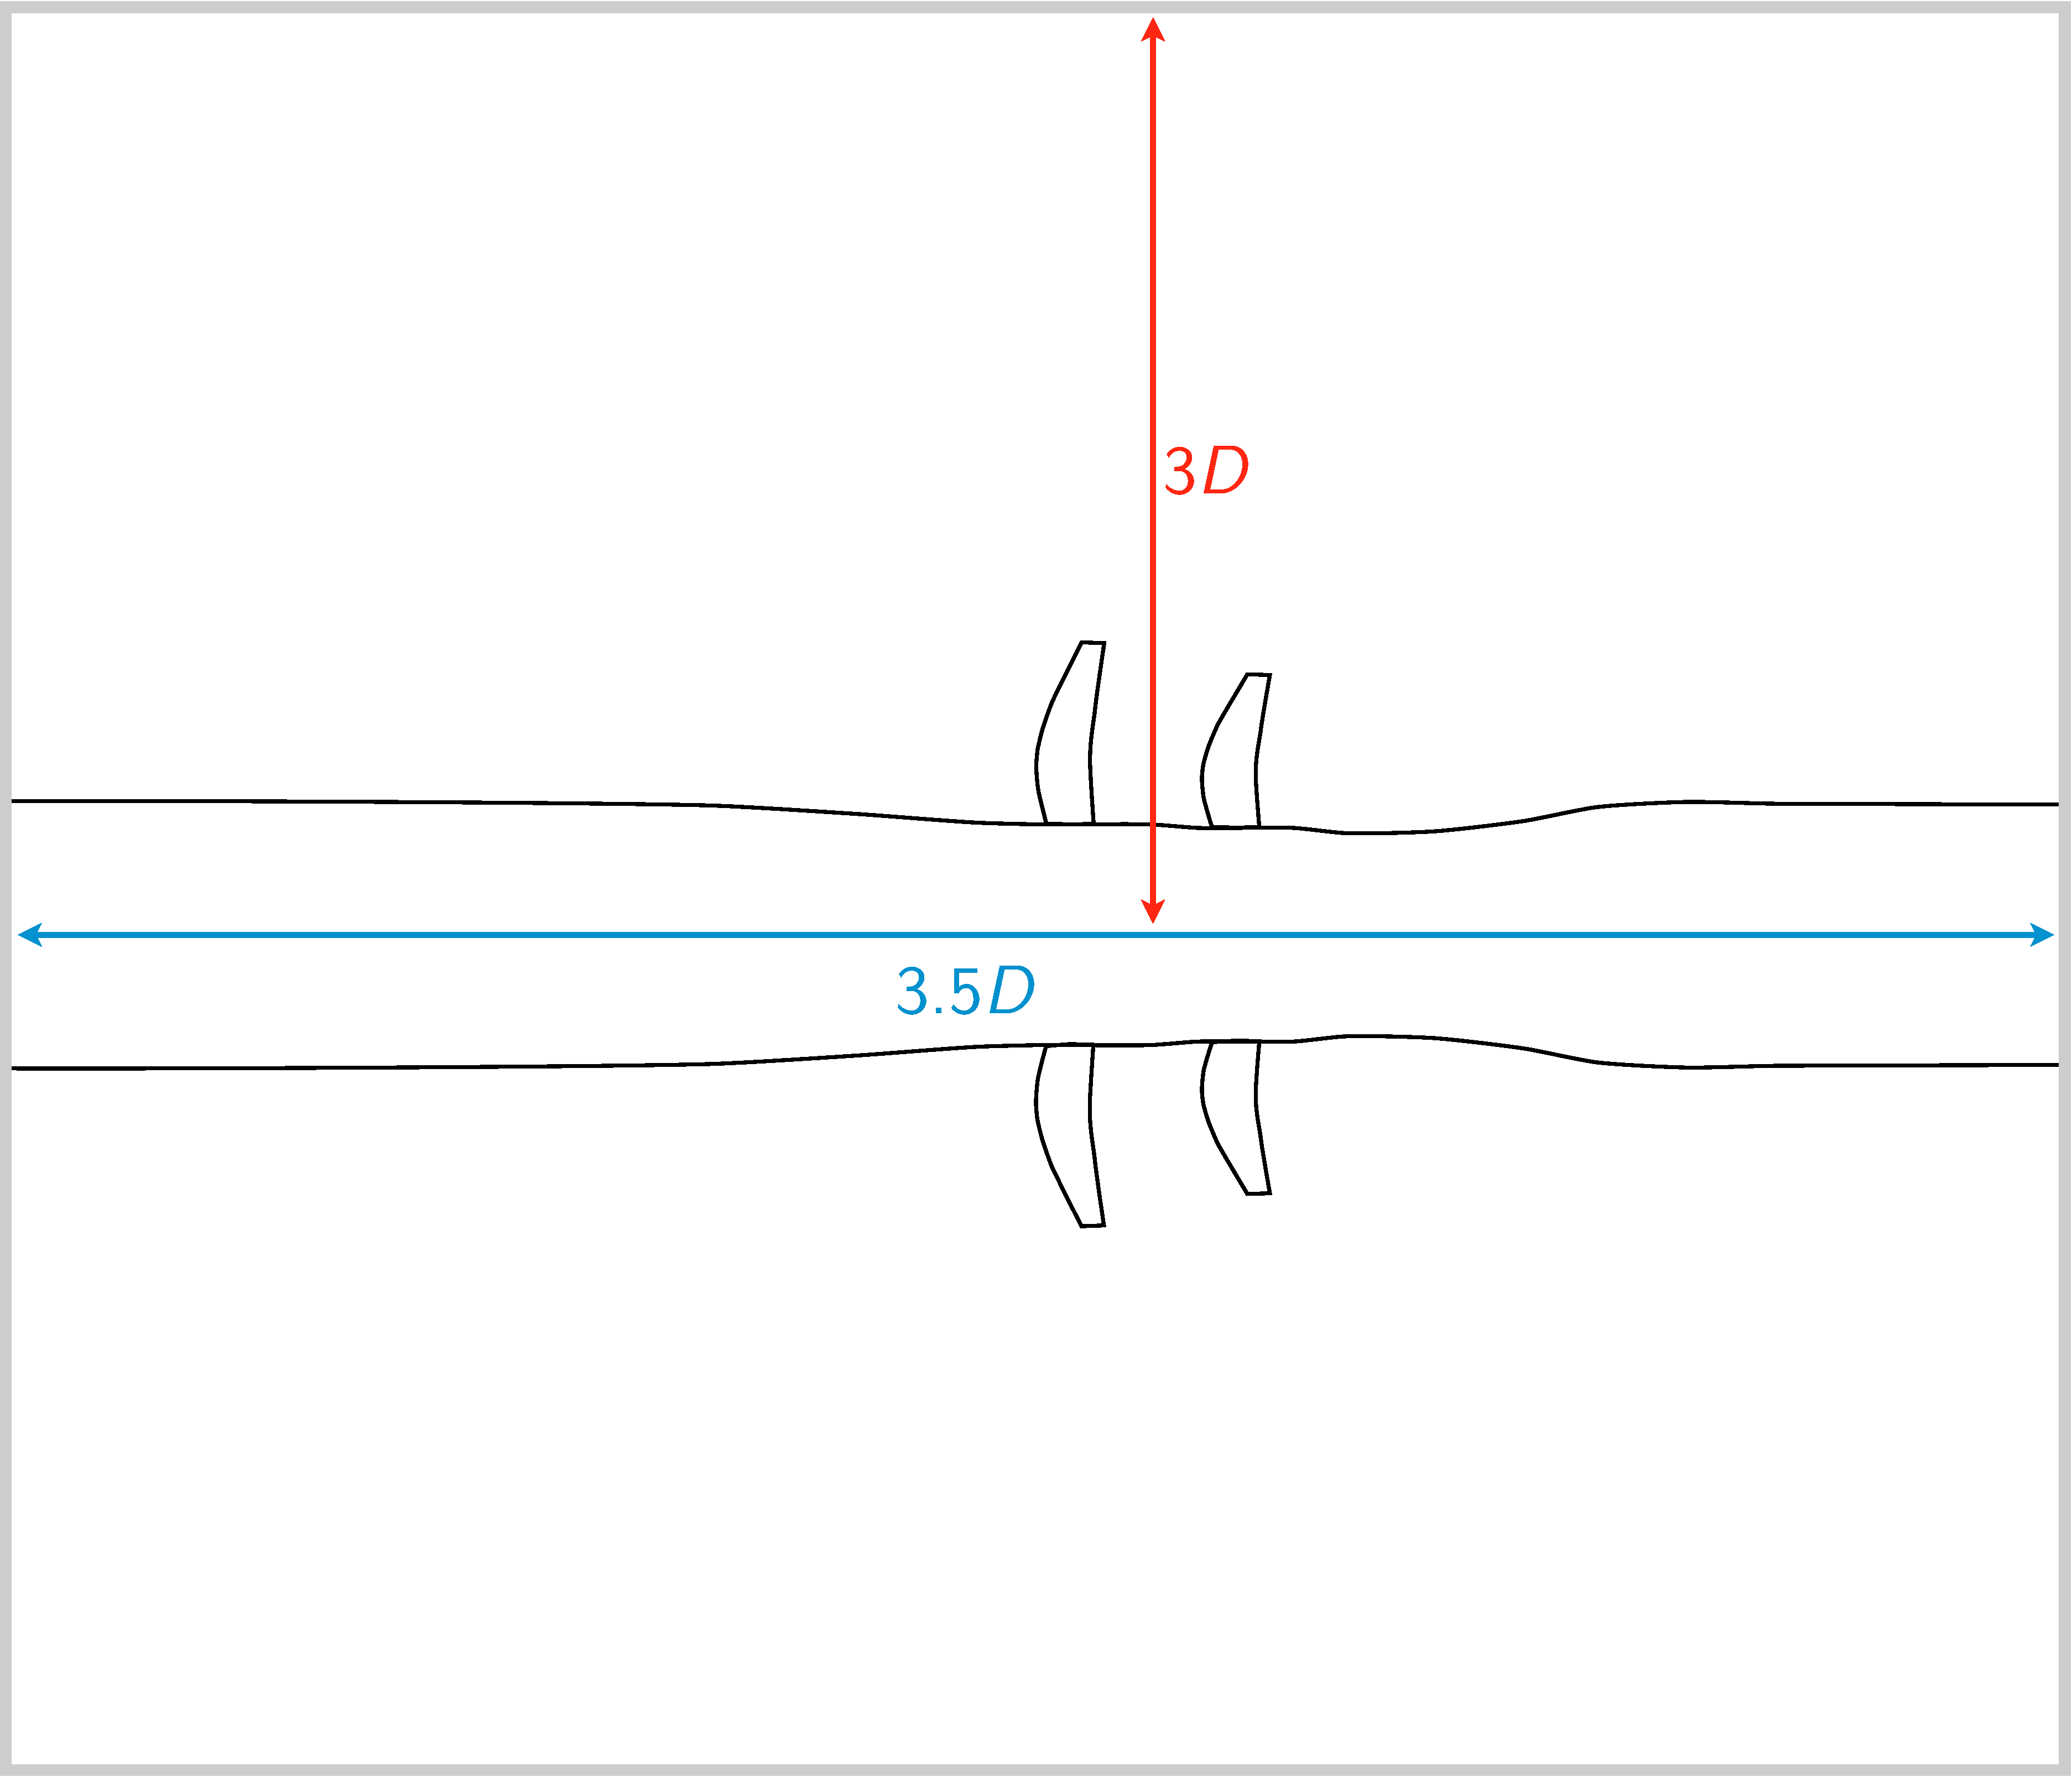
\includegraphics[width=.4\textwidth]{dream_farfield.pdf}
  \caption{Low-speed isolated configuration far-field domain and boundary conditions.}
  \label{fig:dream_farfield}
\end{figure}
As highlighted by underlined text in Fig.~\ref{fig:dream_farfield},
the boundary conditions used are: (i)~adiabatic walls
for the blades and the shroud (or spinner) and (ii)~constant
stagnation values used at the far-field.
In opposite to the study made previously on the STCF11
configuration (see Sec.~\ref{sec:stcf11_numerical}),
the mesh stems from literature and industrial best
practices and thus will not be assessed.

Turbulence is modeled using the one-equation model of
\citet{Spalart1992}.  Roe's scheme~\cite{Roe1981} along with a 
second-order MUSL extrapolation 
is used to compute the convective fluxes.
The maximum CFL number is set to~10 for the steady 
computations and the HB simulations.

\subsection{Influence of the spatial discretization} % (fold)
\label{sub:dream_ls_spatial_discretization}

To assess the influence of spatial discretization, four 
space schemes are used to simulate the low-speed CROR configuration.
These four schemes are the \citet{Jameson1981} scheme (noted JST) with artificial
viscosities $\kappa_4 = 0.016$, $\kappa_4 = 0.032$, $\kappa_4 = 0.064$
and $\kappa_2$ equal to $0.5$ as the operating point should not 
lead to shocks. In addition to this scheme, three upwind
Roe's scheme~\cite{Roe1981} along with no extrapolation (noted Roe~1),
a second order (noted Roe~2) or a third-order (noted Roe~3) 
MUSCL extrapolations are used.

The convergence of the different computations is show 
in Fig.~\ref{fig:dream_ls_space_scheme_residual}
for the four schemes. The convergence is not 
very good. Only the Roe~1 and Roe~2 spatial schemes give 
a convergence that has an acceptable slope. In contrary,
the JST~$\kappa_4 = 0.016$ diverges and the three
remaining schemes hardly converge.
\begin{figure}[htb]
  \centering
  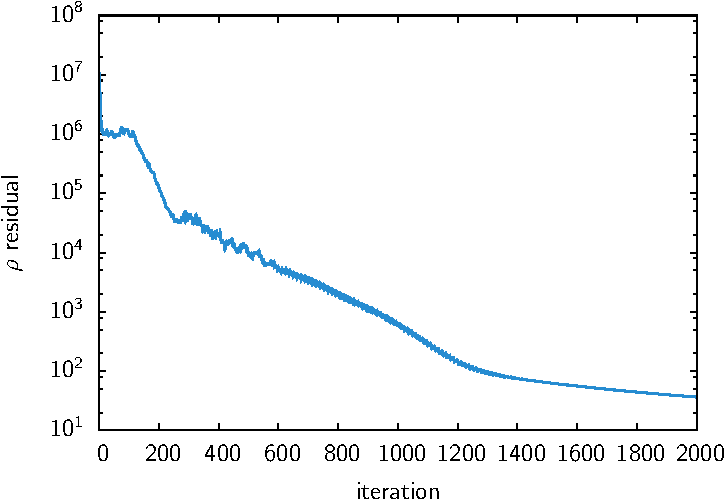
\includegraphics[width=.5\textwidth]{DREAM_LS_RESIDUALS_PPT.pdf}
  \caption{Convergence of the steady computations.}
  \label{fig:dream_ls_space_scheme_residual}
\end{figure}

To differentiate the spatial schemes, 
the steady results for the similarity coefficients are reported
in Fig.~\ref{fig:dream_ls_space_scheme_coeff} for all spatial scheme, 
except the diverging JST~$\kappa_4 = 0.016$ computation.
\begin{figure}[htb]
  \centering
  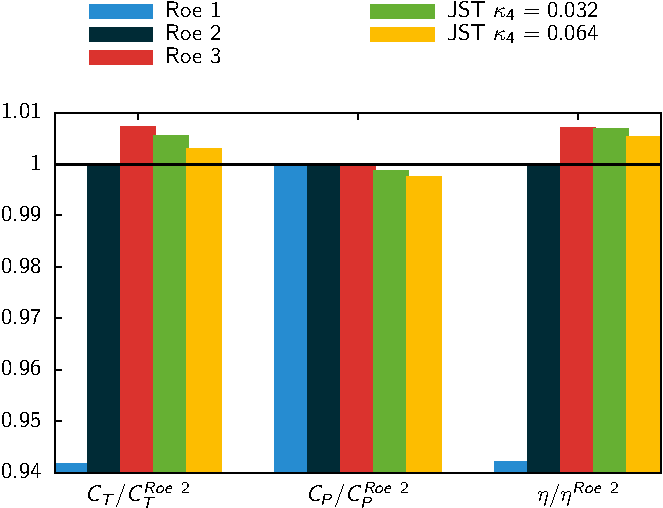
\includegraphics[width=.5\textwidth]{space_scheme_diff.pdf}
  \caption{Convergence of the steady computations, comparison of similarity coefficients.}
  \label{fig:dream_ls_space_scheme_coeff}
\end{figure}
